%% missaali.tex
%% Copyright 2021 Tommi Syrjänen 
%
% This work may be distributed and/or modified under the
% conditions of the LaTeX Project Public License, either version 1.3
% of this license or (at your option) any later version.
% The latest version of this license is in
%   http://www.latex-project.org/lppl.txt
% and version 1.3 or later is part of all distributions of LaTeX
% version 2005/12/01 or later.
%
% This work has the LPPL maintenance status `maintained'.
% 
% The Current Maintainer of this work is Tommi Syrjänen 
%
% See file MANIFEST-Foliono.txt to a list of files that make up this
% work.
\documentclass[a4paper, 12pt]{article}
%% Author: Tommi Syrjänen (tssyrjan@iki.fi)
%%
%% This software is distributed under the LPPL license

%% This is the documentation file for the foliono LaTeX package.
\usepackage{fontspec}
\usepackage{graphicx}

\newcommand{\feature}[1]{\texttt{#1}}
\newcommand{\command}[1]{\texttt{\textbackslash{}#1}}
\newcommand{\commandone}[2]{\texttt{\textbackslash{}#1\{#2\}}}
\newcommand{\commandtwo}[3]{\texttt{\textbackslash{}#1\{#2\}\{#3\}}}
\newcommand{\argument}[1]{\texttt{#1}}

\makeatletter

\newcommand{\foliodemo}[2]{%
  \setfoliono{#1}{#2}%
  \currentfoliowithstyles% 
}

\makeatother



\title{The \texttt{foliono} package \\
  Folio numbering for old books}

\author{Tommi Syrjänen\\ \texttt{tssyrjan@iki.fi}}
\date{Version 1.0, 25 March, 2021}

\usepackage{foliono}


% Define the folionumber font. This font is available in the package
% 'missaali'
\folionofont{Missaali}
\folionofontsize{14}

\begin{document}

\maketitle

\begin{abstract}
  The \texttt{foliono} package implements medieval and early modern
  folio numbering with a few customizable options. In folio numbering
  only every other page gets a number and the number has two parts
  that identify both the quire and the folio inside of the quire. The
  package works best in conjunction with the \texttt{fancyhdr} package
  but it can be used also without it. 
\end{abstract}

\section{Introduction}

Before modern page numbering was introduced, the pages of a book were
numbered using \emph{folio numbering}. In this context \emph{folio}
means a single leaf of a page, an odd page and the even page that is
on the other side of. 

A medieval book was composed of \emph{quires}. A quire is a collection
of sheets of paper or parchment that are folded together to form
pages. As the name suggests, most quires had four sheets that were
folded to form eight folios and 16 pages, but there were also three,
five, and even six sheet quires. With printed books the modern term
\emph{gathering} is usually used in place of \emph{quire}, but I have
used \emph{quire} throughout because it is shorter.

A medieval scribe would write the text on quires and then a bookbinder
would sew the completed quires together and attach the book covers.
Most texts needed more than one quire. Scribes started to number the
quires to help bookbinders to keep the quires in order. They were
usually marked by writing letters in alphabetical order at the bottom
or top right corner of the first page of the quire.

\begin{figure}
  \centering
\begin{verbatim}
\usepackage{foliono}
\usepackage{fancyhdr}
\pagestyle{fancy}
\cfoot{}
\renewcommand{\headrulewidth}{0pt} 
\fancyfoot[R]{\folionumber}
\end{verbatim}
  \caption{Quick-start minimal code skeleton with \feature{fancyhdr}.}
  \label{fig:quick_start}
\end{figure}


Later scribes started to add numbers for the individual folios of a
quire. This was usually done for books that needed a table of contents
or an index. Folio numbering became more prevalent with the advent of
printing as including them helped the bookbinder to ensure that the
sheets were folded right and put in the correct order.

For printed books the quires are formed using two basic principles.
The largest book format is called \emph{folio} and there the sheet is
folded once so that the result has two folios and four pages. These
sheets are collected in quires the same ways as manuscript sheets
were. In late medieval and early modern times the number of sheets put
in a quire varied also for printed books. I have seen examples ranging
from three sheets (6 folios) to six sheets (12 folios), with five
sheets (10 folios) being very common.

In smaller format books one printed sheet usually makes up a quire by
itself. In \emph{quarto} size the sheet is folded twice, so a quire
will have only four folios, in \emph{octavo} it is folded three times
so there are eight folios per quire, and in \emph{duodecimo} sheets
are folded four times to produce 12 folios.

\begin{table}[b]
  \centering
  \begin{tabular}{lcc}
    Format & Folios per quire & Pages per quire \\
    \hline
    Folio (2:o) &  6-12 & 12-24 \\ 
    Quarto (4:o) & 4 & 8 \\
    Octavo (8:o) & 8 & 16 \\
    Duodecimo (12:o) & 12 & 24 \\
  \end{tabular}
  \caption{Common old printed book formats}
  \label{fig:formats}
\end{table}

A medieval or early modern folio number generally consists of two
parts, the quire number (A, B) and the folio number within quire in
Roman numerals (i, ii). There are some examples where the folios are
numbered sequentially from the start with no respect to the quire
structure. In many of these cases the folio numbers were added after
the book had already been bound.

In modern reference convention the
two pages of a folio are called \emph{recto} (r) and \emph{verso} (v).
The recto is the first page of the folio that is shown on the right
hand side of the spread and the verso is the second page on the left
hand side.

Bookprinters often did not include the folio number for each folio of
the quire. For example, with the \emph{folio} and \emph{octavo}
formats it was common that only the folios of the first half of a
quire had numbers. Similarly, with \emph{quarto} the last folio number
of a quire was often left out.

The \feature{foliono} package supports several different folio
numbering conventions and it also provides very rudimentary support
for creating tables of content and indices for folio-numbered
documents. However, a lot of manual work is necessary for creating
them. 

\begin{figure}
  \centering
  \begin{tabular}{cc}
    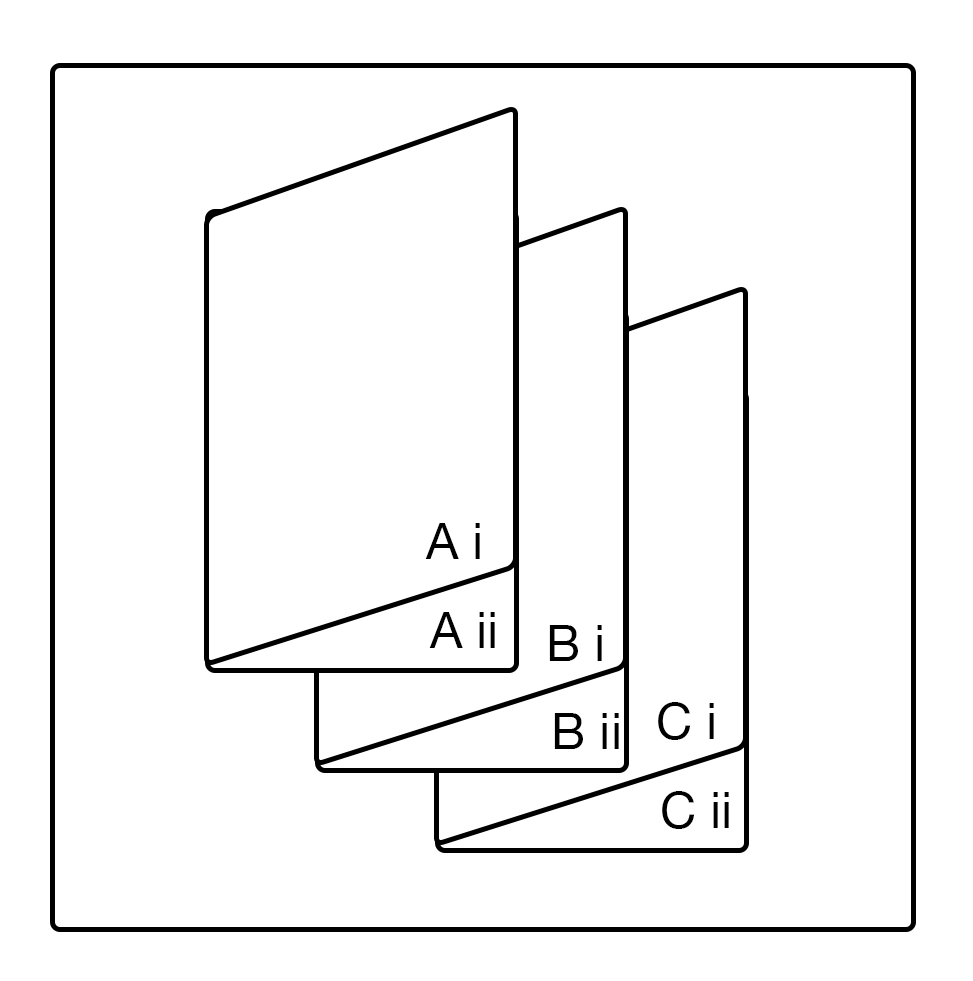
\includegraphics[width=5cm]{pics/standard.png} & 
    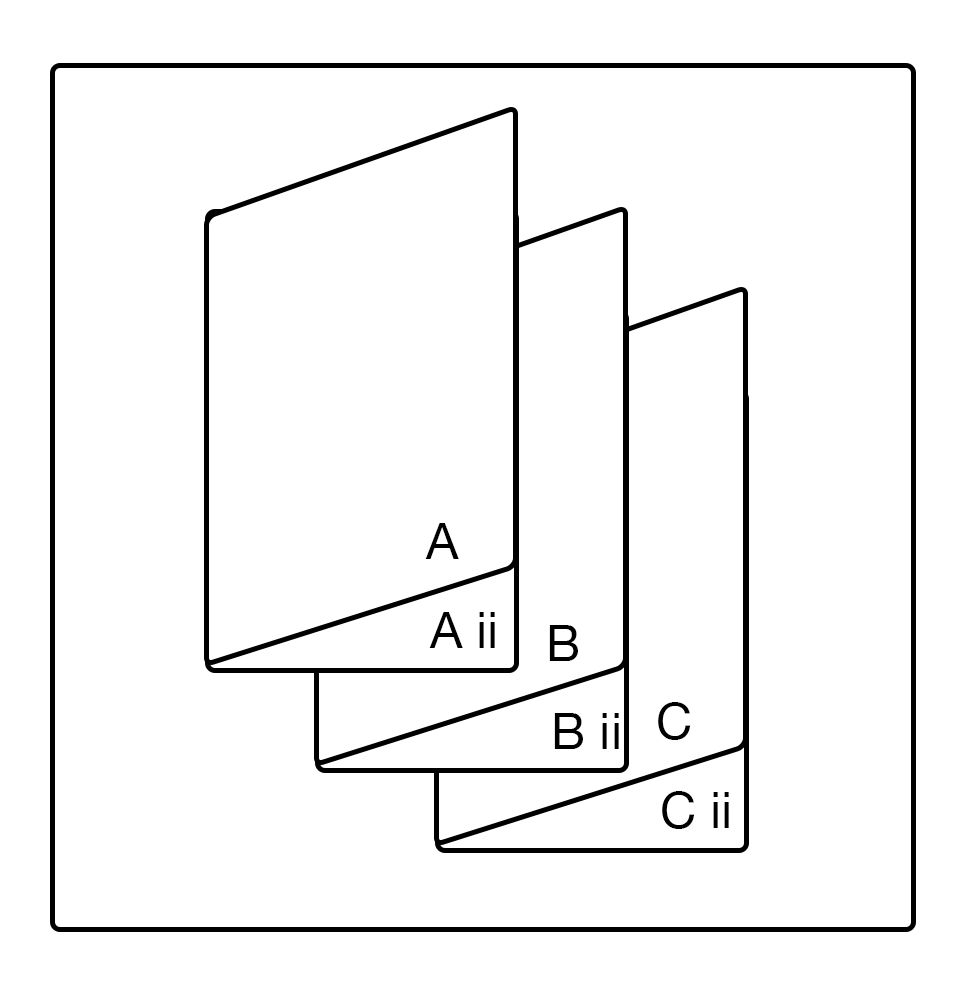
\includegraphics[width=5cm]{pics/skip-first.png} \\
    (a) Default & (b) \feature{SkipFirst} \\
    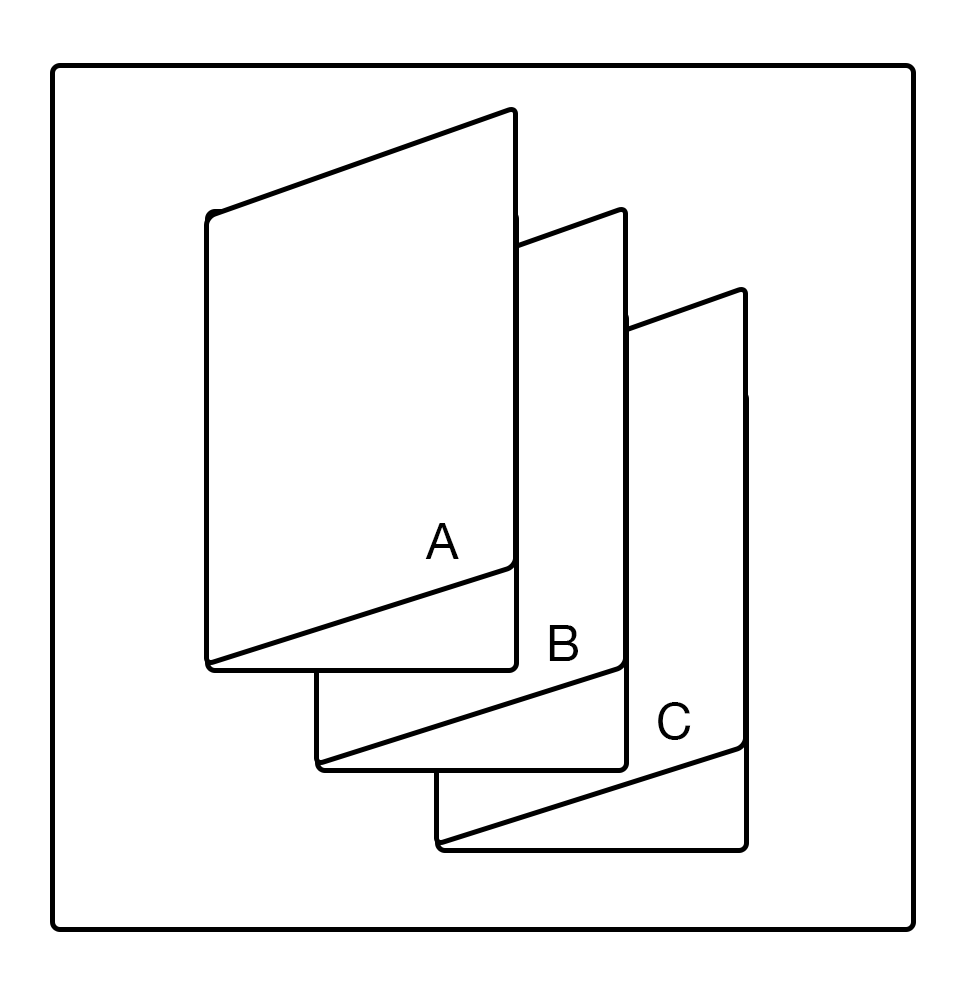
\includegraphics[width=5cm]{pics/only-quire.png} & 
    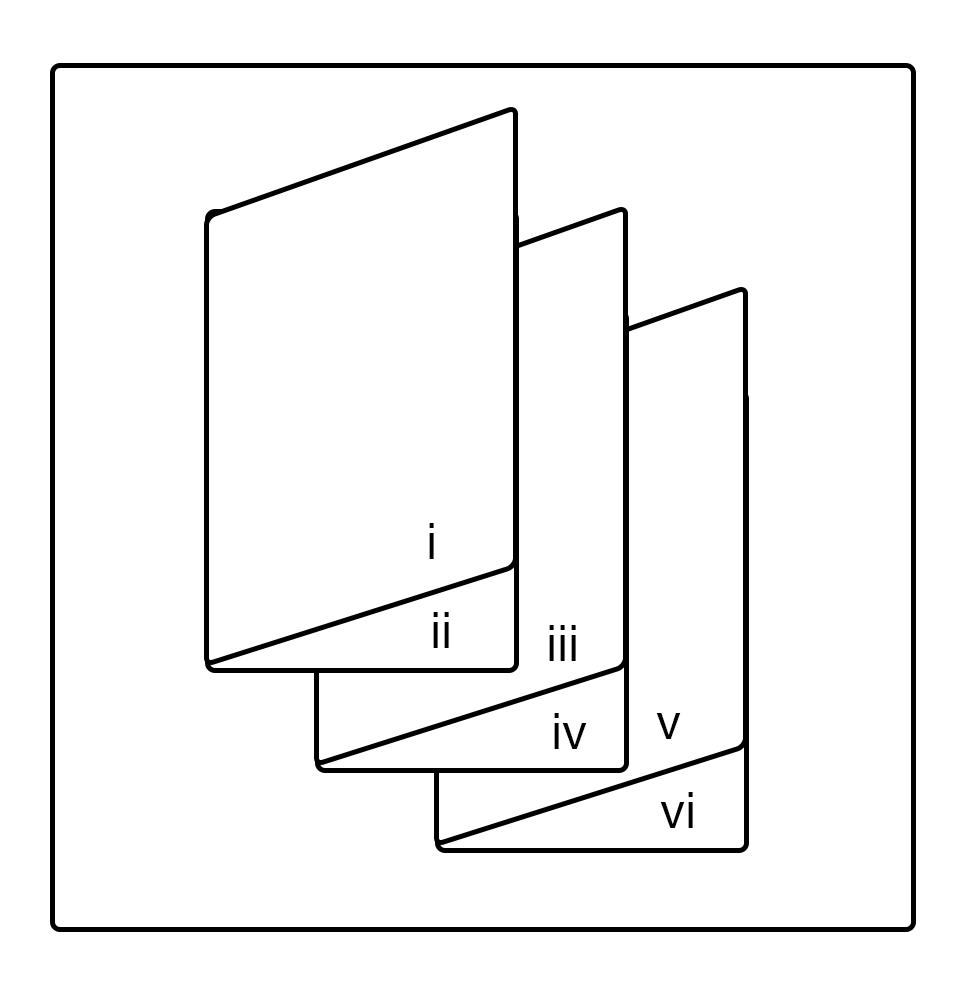
\includegraphics[width=5cm]{pics/only-folio} \\
    (c) \feature{OnlyQuire} & (d) \feature{NoQuires} \\
  \end{tabular}
  \caption{Mode of operation samples}
  \label{fig:modes}
\end{figure}

In the examples I will be using the font \emph{Missaali} to typeset
the folio numbers as they would appear on the page. \emph{Missaali} is
a free opentype font that comes with the package \feature{missaali}
that is based on late 15th century book Northern German book textura. 

\section{Modes of operation}
 
The \feature{foliono} package can operate in several different modes
that are controlled using the package options. A folio number consists
of two parts, the quire number and the folio number, and the different
modes show them using different principles. Figure \ref{fig:modes}
shows four of the basic modes in schematics. 

\begin{description}
\item [Default] \mbox{} \\
  The default behavior of \emph{foliono} is that each folio is
  numbered with both the quire number and the folio number inside a
  quire. Thus, the folio numbers advance like:
  \begin{center}
    A 1, A 2, \textellipsis, A 8, B 1, B 2, \textellipsis, B 8, C 1, \textellipsis
  \end{center}
  
\item [Skip first folio number (\feature{SkipFirst})] \mbox{} \\
  The first folio number skipping mode is otherwise the same as the
  default mode, but the first folio of a quire contains only the quire
  number and not the folio counter. The numbers advance like:
  \begin{center}
    A, A 2, A 3, \textellipsis, A 8, B, B 2, \textellipsis, C , C 2 \textellipsis
  \end{center}


  
\item [Only quire numbers (\feature{OnlyQuire})] \mbox{}\\
  In the only quire numbers mode the folio numbers are not included
  at all and only the first pages of a quire have the mark:
  \begin{center}
    A, \{\}, \{\}, \{\}, \{\}, \{\}, \{\}, \{\}, B, \{\}, \textellipsis
  \end{center}
  
\item [No quires (\feature{NoQuires})]\mbox{} \\
  In this mode the folios are numbered sequentially from the start of
  the book paying no regards to the quire structure. Here the numbers
  are simply:
  \begin{center}
    1, 2, 3, 4, 5, \textellipsis
  \end{center}

\item [Sheet numbering (\feature{SheetNumbering})] \mbox{}\\
  In sheet numbering mode there is only one folio number per a two
  page sheet. In practice, this means that the first half folios of a
  quire are numbered using the default style and the latter half are
  left unnumbered:
  \begin{center}
    A 1, A 2, A 3, A 4, \{\}, \{\}, \{\}, \{\}, B 1, B 2, \textellipsis
  \end{center}
  This mode can be combined with skipping the first folio number. 


\item [Skip end half (\feature{SkipEnd})] \mbox{} \\
  In this mode the folio numbers are printed to the first half + 1
  folios of a quire and the rest are left empty. In practice the
  effect is otherwise same as with sheet numbering except that one
  more folio has a number.

  For quarto format the numbers go:
  \begin{center}
    A 1, A 2, A 3,  \{\}, B 1, B 2, \textellipsis
  \end{center}
  For octavo format the numbers are:
  \begin{center}
    A 1, A 2, \textellipsis, A 5,  \{\},  \{\},  \{\}, B 1, B 2, \textellipsis
  \end{center}
  For duodecimo they go:
  \begin{center}
    A 1, A 2, \textellipsis, A 7,  \{\},  \{\},  \{\}, \{\}, \{\}, B 1, B 2, \textellipsis
  \end{center}
  This mode can be combined with skipping the first folio number.   

\end{description}

\section{General usage}

The basic command in the package is \command{folionumber}. This should
be put either in the header or footer of the page and it should be run
exactly once on each page since it keeps track of the folio number
counters and also whether we are on recto or verso side of the folio.
Manipulating headers and footers is simplest with the
\feature{fancyhdr} package. For the basic functionality you can add
the following to the preamble of the document:

\begin{verbatim}
\usepackage{fancyhdr}
\usepackage{foliono}
\cfoot{}
\renewcommand{\headrulewidth}{0pt}
\fancyfoot[R]{\folionumber}
\pagestyle{fancy}
\end{verbatim}

Here the \command{cfoot} removes the modern page number,
\command{fancyfoot} adds the folio number to the right footer,
overriding the \command{headrulewidth} removes the horizontal line
from top that \feature{fancyhdr} wants to add there, and
\command{pagestyle} enables the fancy header style.

You need to decide how big your quires are. The package defaults to
eight folio quires, meaning that when printed there are four sheets in
the quire. Historically that was the most common quire size for
manuscripts, but other sizes were also used. You can set the quire
size with the \command{folionoquirefolios} command. For example:
\begin{verbatim}
\folionoquirefolios{10}
\end{verbatim}
sets the quires to have 10 folios and 20 pages each. It is possible to
change the value in the middle of the document to get quires of
different sizes. 

In case you need to set the folio number manually, there are two ways
to do it:

\begin{enumerate}
\item \command{stepfolio}: this moves the counters to the next folio.
\item \commandtwo{setfoliono}{quireNo}{folioNo}: sets the quire
  counter to \argument{quireNo} and the folio counter to
  \argument{folioNo}. 
\end{enumerate}

There are three commands that you can use to access the current folio
number from text. All of these commands set the folio number even if
\command{folionumber} does not print it on the page.
\begin{enumerate}
\item \command{currentfolio} this sets the current folio number as
  unformatted string. 

\item \command{currentfoliowithsides} this sets the current folio
  number as unformatted string that is followed by the side reference
  \feature{r} or \feature{v}. 

\item \command{currentfoliowithstyles} this sets the current folio
  number formatted and styled the exact same way as it is  

\end{enumerate}

Here is an example for their use:

\begin{center}
\begin{tabular}{lc}
    \begin{minipage}{0.5\linewidth}
\begin{verbatim}
\setfoliono{2}{4}
1: \currentfolio \\
2: \currentfoliowithsides \\
3: \currentfoliowithstyles \\
\end{verbatim}
    \end{minipage}
&
    \begin{minipage}{0.4\linewidth}
      \setfoliono{3}{4}\strut\mbox{}\\
      \strut\mbox{}\\
      1: \currentfolio \\
      2: \currentfoliowithsides \\
      3: \currentfoliowithstyles \\
      \end{minipage}
  \end{tabular}
\end{center}

\subsection{Font selection and properties}

By default the folio numbers are set using the default document font
and size. There are commands that allow you to select the font when
using the \feature{fontspec} package. If you are using some other
environment, you can redefine the \command{folionostyle} command that
adds style to the folio numbers.

The font selection commands are:
\begin{enumerate}
\item \commandone{folionofont}{FontName}: set the \feature{fontspec}
  font that is used to set the folio number. You need to set this for
  the other two font setting commands having effect.

\item \commandone{folionofontsize}{size}: set the size of the folio
  number. The font must have been set eariler. 

\item \commandone{folionofontcolor}{color}: set the color for the
  folio number. The font must have been set eariler.

\end{enumerate}

\begin{center}
  \begin{tabular}{lc}
    \begin{minipage}{0.6\linewidth}
\begin{verbatim}
Before: \currentfoliowithstyles \\
\folionofont{Missaali}
\folionofontsize{18}
\folionofontcolor{c55e47}
After: \currentfoliowithstyles 
\end{verbatim}
    \end{minipage}
    &
    \begin{minipage}{0.3\linewidth}
      \begingroup
      Before: \currentfoliowithstyles \\
      \folionofont{Missaali}
      \folionofontsize{18}
      \folionofontcolor{c55e47}
      After: \currentfoliowithstyles 
      \folionofontsize{14}
      \folionofontcolor{000000}
      \endgroup
    \end{minipage}
  \end{tabular}
\end{center}

\subsection{Controlling the formatting}

By default the folio number is typeset with a space between the quire
and folio numbers. There are commands to add content or commands
before and after the both commands as well as to override the default
separator. 

\begin{enumerate}
\item \commandone{quirenoprefix}{text}: the \emph{text} is added
  before the quire number.
\item \commandone{quirenosuffix}{text}: the \emph{text} is added
  after the quire number.
\item \commandone{folionoprefix}{text}: the \emph{text} is added
  before the folio number.
\item \commandone{folionosuffix}{text}: the \emph{text} is added
  after the folio number.
\item \commandone{folionoseparator}{text}: the \emph{text} is added
  between the quire and folio numbers. 
\end{enumerate}

\begin{figure}
  \centering
\begin{verbatim}
\quirenostyle{%
  \quirenoprefix%
  QUIRE COUNTER%
  \quirenosuffix%
  \folionoseparator}%
\folionostyle{%
  \folionoprefix%
  FOLIO COUNTER%
  \folionosuffix%
}
\end{verbatim}
  \caption{A pseudocode explanation on how the quire number is
    formatted. The separator is formatted using the quire number
    style.}
  \label{fig:foliono}
\end{figure}
For example, you can add periods before, after, and in the middle of
the folio number with:
\begin{center}
  \begin{tabular}{lc}
    \begin{minipage}{0.6\linewidth}
\begin{verbatim}
\quirenoprefix{.}
\folionoseparator{.}
\folionosuffix{.}
\currentfoliowithstyles
\end{verbatim}
    \end{minipage}
    &
    \begin{minipage}{0.3\linewidth}
       \quirenoprefix{.}
       \folionoseparator{.}
       \folionosuffix{.}
       \currentfoliowithstyles
       \quirenoprefix{}
       \folionosuffix{}
       \folionoseparator{\hbox{ }}
    \end{minipage}
  \end{tabular}
\end{center}

You can also add formatting commands to the prefixes. For example, you
can achieve two-colored folio numbers with:
\begin{verbatim}
\quirenoprefix{\addfontfeature{Color=455f9b}}
\folionoprefix{\addfontfeature{Color=c55e47}}
\currentfoliowithstyles
\end{verbatim}
This produces the result:
\begin{center}
  \begin{minipage}{0.3\linewidth}
    \quirenoprefix{\addfontfeature{Color=455f9b}}
    \folionoprefix{\addfontfeature{Color=c55e47}}
    \currentfoliowithstyles
    \quirenoprefix{}
    \folionoprefix{}
    \end{minipage}
\end{center}

\subsection{Labels and indices}

There are two commands for creating labels that have folio numbers for
the reference and two commands for creating index entries. The basic
forms of the commands typeset the folio numbers without formatting or
prefixes and suffixes, and the two others typeset the numbers as they
appear on page. All of these commands produce the folio number string
even if it is not printed on the current page. Note that commands that
are read in from auxiliary and index files break easily and often
cause weird error messages.

If you want to create a medieval-styled table of contents, the best
way to proceed is probably to use the indexing commands, copy the
index file as a base for a new LaTeX document, and then manipulate
them by hand to get the desired outcome. You can then combine the
original document and the index using the \feature{pdfpages} package.
There are two main reasons to do it this way: as far as I know there
are no existing index formats that would produce results that are even
remotely close to medieval tables of contents or indices, and the main
text should start on the folio A 1 of the document. If the table of
contents is at the beginning, it should be on a separate unnumbered
sheet.

\begin{enumerate}
\item \commandone{folionolabel}{label}: defines a label whose
  reference string is unformatted version of the current folio number.

\item \commandone{folionolabelwithstyles}{label}: defines a label
  whose reference string is the formatted version of the current folio
  number.

\item \commandone{folionoindex}{text}: adds \feature{text} as an index
  entry in the index file.\footnote{Remember to use
    \command{makeindex} command in the preamble if you use index
    commands.}

\item \commandone{folionoindexwithstyles}{text}: adds \feature{text}
  as an index entry in the index file with complete styling.

\end{enumerate}








\section{Package options}

The \feature{foliono} package defines the following options:

\begin{description}
\item [\feature{AllQuires}] \mbox{} \\
  Before the 17th century the letters \emph{i} and \emph{j} were not
  yet separated and they were considered to be two variant forms of
  the same letter that could be used almost interchangeably.
  Similarly, \emph{u} and \emph{v} were still the same. Because of
  this \feature{foliono} does not use \emph{i} and \emph{u} as quire
  numbers by default. The package option \feature{AllQuires} takes the
  two missing letters in use as quire numbers.

\item [\feature{ArabicNumbers}] \mbox{} \\
  This option changes the folio numbers into Arabic numerals instead
  of the Roman numberals. This is most useful together with the
  \feature{NoQuires} option. However, some later printed books used
  Arabic numerals in folio numbers.
  
  \item [\feature{LowerCase}] \mbox{} \\
    This changes the quire numbers to be in lower case instead of the
    default upper case letters. 
    
  \item [\feature{NoQuires}] \mbox{} \\
    This turns on the no quires mode where folio numbers are numbered
    sequentially from one upwards with no regard to quire structure. 

  \item [\feature{OnlyQuire}] \mbox{} \\
    This turns on the only quires mode where folio numbers are left out
    and the quires have a quire number on their first page. 
  
  \item [\feature{SheetNumbers}] \mbox{} \\
    This turns on sheet numbering mode where there is only one folio
    number on a two-folio sheet of paper. In practice the first half
    of folios on a quire will have a number and the rest are empty.
    This does not work together with \feature{NoQuires}.

  \item [\feature{ShowSides}] \mbox{} \\
    If enabled, it will add the indicator \emph{r} or \emph{v} to
    labels and index entries to show if they land on recto or verso
    side of the folio. This is not added to the folio numbers printed
    on pages, only on the references. 

  \item [\feature{SkipFirst}] \mbox{} \\
    When enabled the first folio of a quire will have only the quire
    number and not the folio number. 


  \item [\feature{SkipEnd}] \mbox{} \\
    When enabled the folio numbers are printed on first half + 1
    folios of a quire. The effect is otherwise the same as with
    \feature{SheetNumbers} except that one more folio has the number.
\end{description}

\section{Command Reference}


\begin{description}
\item [\command{folionumber}] \mbox{} \\
  Sets both the formatted and styled folio number to the page and it
  also keeps track of the quire and folio counters as well as the
  recto and verso sides on the document. It should be run exactly once
  per page of output.

\item [\commandone{folionoquirefolios}{folioNo}] \mbox{} \\
  Sets the size of quires to \argument{folioNo} folios.
  The value should be even. This can be run multiple times inside a
  document to get quires of different sizes.

\item [\commandone{folionofont}{fontId}] \mbox{} \\
  Sets the font that is used to folio numbers to the
  \feature{fontspec} font \argument{fontId}. If you are using some
  other font system, you need to redefine \command{folionostyle} and
  \command{quirenostyle} instead.
  
\item [\commandone{folionofontsize}{points}] \mbox{} \\
  Sets the size of the folio number font to \argument{points}. This
  has an effect only if the font has been selected with
  \command{folionofont}. Default size is 10 points. 

\item [\commandone{folionofontcolor}{color}] \mbox{} \\
  Sets the folio number font color to \argument{color}. This has an
  effect only if the font has been selected with
  \command{folionofont}. Default color is black. 

\item [\commandone{quirenostyle}{commands}] \mbox{} \\
  A styling command for non-\feature{fontspec} users. Redefine this
  command to apply styling to the quire counter. This defaults to
  using the font, size, and color set using the previous font
  selection commands.

\item [\commandone{folionostyle}{commands}] \mbox{} \\
  A styling command for non-\feature{fontspec} users. Redefine this to
  apply styling to the folio counter. This defaults to using the font,
  size, and color set using the previous font selection commands.

\item [\commandone{folionolabel}{label}] \mbox{} \\
  Adds a \argument{label} that can be accessed with the \command{ref}
  command. The label text will be an unformatted folio number string.
  This creates a reference using the folio number of that particular
  page even if the number is not printed on the page. This has the
  most obvious effect when the \feature{SheetNumbers} option is turned
  on.

\item [\commandone{folionolabelwithstyles}{label}] \mbox{} \\
  Adds a \argument{label} whose reference text contains all the styles
  and formatting of the current folio number. Otherwise this works the
  same as \command{folionolabel}. \emph{Note! It is very easy to get
    weird TeX error messages if there is anything complex or fragile
    in the commands read from .aux files}.

\item [\commandone{folionoindex}{text}] \mbox{} \\
  This adds \argument{text} as an index entry where the page number is
  replaced with unformatted current folio number. Using this command
  and some manual manipulation is the easiest way to create medieval
  tables of context. 

\item [\commandone{folionoindexwithstyles}{text}] \mbox{} \\
  This adds \argument{text} as an index entry where the page number is
  replaced with styled current folio number. 

\item [\commandtwo{setfoliono}{quireNo}{folioNo}] \mbox{} \\
  Sets the quire counter to \argument{quireNo} and the folio counter
  to \argument{folioNo}.

\item [\command{stepfolio}] \mbox{} \\
  Moves the folio number to the next folio. This is most useful in
  cases you want to remove the folio number from a single page as
  setting the page style to \argument{empty} also prevents
  \command{folionumber} from moving to the next number.

\item [\commandone{quirenoprefix}{text}] \mbox{} \\
  Sets a prefix of the quire number to be \argument{text}. The prefix
  can contain formatting commands, but the more complex the commands
  are, the more likely is that \command{folionolabelwithstyles} and
  \command{folionoindexwithstyles} commands break. 

\item [\commandone{quirenosuffix}{text}] \mbox{} \\
  Sets the quire number suffix to \argument{text}. The suffix may
  contain both text and commands.

\item [\commandone{folionoprefix}{text}] \mbox{} \\
  Sets the folio counter prefix to \argument{text}. 

\item [\commandone{folionosuffix}{text}] \mbox{} \\
  Sets the folio number suffix to \argument{text}. 

\item [\commandone{folionoseparator}{text}] \mbox{} \\
  Sets the separator that is placed between quire and folio numbers to
  \argument{text}. The separator is formatted according to the quire
  number style. 

\item [\command{currentfolio}] \mbox{} \\
  Gives the unformatted and non-styled version of the current folio
  number. In particular, the prefixes, suffixes, and the separator are
  left out of it.

\item [\command{currentfoliowithsides}] \mbox{} \\
  Gives the unformatted and non-styled version of the current folio
  number with the side indicator (\emph{r} or \emph{v}) added to its
  end.

\item [\command{currentfoliowithstyles}] \mbox{} \\
  Gives the current folio number formatted the same way as it is added
  to the page by \command{folionumber}. This gives the real folio
  number even if \command{folionumber} will skip it, for example, if
  we are in the second half of a quire and \feature{SheetNumbers} is
  turned on.


\end{description}

\section{Examples}

\begin{description}
  
\item [Codex Montpellier, c.1300] \mbox{} \\
  \begin{tabular}{lp{7cm}}
    Author: & unknown \\
    Format: & manuscript \\
    Folio numbers: & continuously running folio numbers, roman numbers
    surrounded by centered dots.  \\
    Sample: &
    \begin{minipage}{7cm}
      \makeatletter
      \FolioNo@noQuirestrue
      \folionoprefix{·}
      \folionosuffix{·}
      \folionoseparator{}
      \foliono@createFormattedFolioLabel      
      \folionoprefix{}
      \folionosuffix{}
      \folionoseparator{\hbox{ }}
      \makeatother
    \end{minipage} \\
  \end{tabular}

  Code:

  \begin{minipage}{5cm}
    \verb!\usepackage[NoQuires]{foliono}!\\
    \verb!\folionoprefix{·}! \\
    \verb!\folionosuffix{·}! \\
  \end{minipage}
  

\item [Glogauer Liederbuch, c. 1480] \mbox{} \\
  \begin{tabular}{lp{7cm}}
    Author: & unknown \\
    Format: & manuscript \\
    Folios: & 12 per quire \\
    Folio numbers: & on top right of every folio, most quires have
    lower case quire numbers but some use upper case \\
    Sample: &
    \begin{minipage}{6cm}
      \makeatletter
      \Foliono@capitalizeQuireNumberfalse
      \foliono@createFormattedFolioLabel      
      \makeatother
    \end{minipage} \\
  \end{tabular}

  Code: 

  \begin{minipage}{5cm}
    \verb!\usepackage[LowerCase]{foliono}!\\
    \verb!\folionoquirefolios{12}!\\
  \end{minipage}

\item [Missale Aboense, 1488] \mbox{} \\
  \begin{tabular}{lp{7cm}}
    Bookprinter: & Barthomolew Ghotan \\
    Format: & folio \\
    Folios: & 12 per quire \\
    Folio numbers: & on every folio, capital quire number, centered dots surround  folio number \\
    Sample: &
    \begin{minipage}{6cm}
      \folionoprefix{·}
      \folionosuffix{·}
      \folionoseparator{}
      \currentfoliowithstyles
      \folionoprefix{}
      \folionosuffix{·}
      \folionoseparator{\hbox{ }}
    \end{minipage} \\
  \end{tabular}

  Code:

  \begin{minipage}{5cm}
    \verb!\usepackage{foliono}!\\
    \verb!\folionoquirefolios{12}!\\
    \verb!\folionoprefix{·}! \\
    \verb!\folionosuffix{·}! \\
    \verb!\folionoseparator{}!
  \end{minipage}

  
\item [Revelationes Sancti Birgitte, 1492] \mbox{} \\
  \begin{tabular}{lp{7cm}}
    Bookprinter: & Barthomolew Ghotan \\
    Format: & folio \\
    Folios: & 10 per quire \\
    Folio numbers: & on first half of a quire, lower case quire number, periods surround  folio number \\
    Sample: &
    \begin{minipage}{6cm}
      \makeatletter
      \Foliono@capitalizeQuireNumberfalse
      \makeatother
      \folionoprefix{.}
      \folionosuffix{.}
      \folionoseparator{}
      \currentfoliowithstyles
      \folionoprefix{}
      \folionosuffix{}
      \folionoseparator{\hbox{ }}
    \end{minipage} 
  \end{tabular}  

Code:

\begin{minipage}{5cm}
  \verb!\usepackage[LowerCase,SheetNumbers]{foliono}!\\
  \verb!\folionoquirefolios{10}!\\
  \verb!\folionoprefix{.}! \\
  \verb!\folionosuffix{.}! \\
  \verb!\folionoseparator{}!
\end{minipage}

\item[Messu eli Herran Echtolinen, 1549] \mbox{} \\
  \begin{tabular}{lp{7cm}}
    Author: & Mikael Agricola \\
    Format: & quarto \\
    Folios: & 8 per quire \\
    Folio numbers: & first folio of a quire has only quire number,
    quire numbers are capitalized. \\
    Sample: &
    \begin{minipage}{6cm}
      \currentfoliowithstyles
    \end{minipage} 
  \end{tabular}  

Code:

\begin{minipage}{5cm}
  \verb!\usepackage[SkipFirst]{foliono}!\\
  \verb!\folionoquirefolios{8}!\\
\end{minipage}

\item[Historiae animalum, 1551] \mbox{} \\
  \begin{tabular}{lp{7cm}}
    Author: & Conrad Gessner \\
    Format: & folio \\
    Folios: & 6 or 8 per quire \\
    Folio numbers: & quire numbers are set in Roman typeface, most are
    upper case but preface uses lower case, folio
    numbers with arabic numbers, only one folio number per sheet.
    \\
    Sample: &
    \begin{minipage}{6cm}
      \makeatletter
      \def\quirenostyle{}
      \def\folionostyle{}
      \FolioNo@useSheetNumberingtrue
      \FolioNo@UseArabicNumberstrue
      \setfoliono{3}{2}
      \makeatother
      \currentfoliowithstyles
    \end{minipage} 
  \end{tabular}  

  Code: 

\begin{minipage}{5cm}
  \verb!\usepackage[SheetNumbers,ArabicNumbers]{foliono}!\\
  \verb!\folionoquirefolios{6}!\\
\end{minipage}



\item[Wanhain Suomen maan Pijspain Latinan kielised laulud, 1616] \mbox{} \\
  \begin{tabular}{lp{7cm}}
    Author: & Hemminki Maskulainen \\
    Format: & octavo \\
    Folios: & 8 per quire \\
    Folio numbers: & folio numbers on first five folios of a quire,
    the first folio has just the quire number, quire number in upper
    case.  \\
    Sample: &
    \begin{minipage}{6cm}
      \makeatletter
      \setfoliono{3}{4}
      \FolioNo@skipFirstFolioNumbertrue
      \FolioNo@onlyFirstHalftrue
      \makeatother
      \currentfoliowithstyles
    \end{minipage} 
  \end{tabular}  

Code:

\begin{minipage}{5cm}
  \verb!\usepackage[SkipFirst,SkipEnd]{foliono}!\\
  \verb!\folionoquirefolios{8}!\\
\end{minipage}


\item[Somen Kielinen Catechismus, 1628] \mbox{} \\
  \begin{tabular}{lp{7cm}}
    Author: & Martin Luther \\
    Translator: &  Knut Carelius \\
    Format: & quarto \\
    Folios: & 4 per quire \\
    Folio numbers: & first folio of a quire has only quire number,
    last folio of a quire is without number, 
    quire numbers are capitalized. \\
    Sample: &
    \begin{minipage}{6cm}
      \currentfoliowithstyles
    \end{minipage} 
  \end{tabular}  

Code:

\begin{minipage}{5cm}
  \verb!\usepackage[SkipFirst,SkipEnd]{foliono}!\\
  \verb!\folionoquirefolios{4}!\\
\end{minipage}


\end{description}





\end{document}
